% ==============================================================================
% CỤM 1 - ĐỀ THAM KHẢO 1 (NĂM HỌC 2026 - 2027)
% ==============================================================================

\begin{bt}%[9D6H18-2]
% nguon: Đề tham khảo Tuyển sinh 10 TP.HCM 2026-2027 – Cụm 1 (Đề 1), Bài 1, trang 3
Cho hàm số $(P): y = \dfrac{x^2}{4}$.
\begin{enumerate}[a)]
	\item Vẽ đồ thị $(P)$.
	\item Tìm điểm $K$ thuộc $(P)$ có tung độ nhỏ hơn hoành độ $1$ đơn vị.
\end{enumerate}
\loigiai{
	\begin{enumerate}[a)]
		\item Bảng giá trị tương ứng giữa $x$ và $y$:
		\begin{center}
		\begin{tabular}{|c|c|c|c|c|c|}
		\hline
		$x$ & $-4$ & $-2$ & $0$ & $2$ & $4$ \\
		\hline
		$y = \dfrac{x^2}{4}$ & $4$ & $1$ & $0$ & $1$ & $4$ \\
		\hline
		\end{tabular}
		\end{center}
		Đồ thị $(P)$ là đường cong parabol đi qua gốc tọa độ $O(0; 0)$ và các điểm $(-4; 4)$, $(-2; 1)$, $(2; 1)$, $(4; 4)$, nhận trục tung $Oy$ làm trục đối xứng.
		\begin{center}
		\begin{tikzpicture}[>=stealth, scale=0.8]
			\draw[->] (-5,0) -- (5,0) node[below] {$x$};
			\draw[->] (0,-0.5) -- (0,5.5) node[left] {$y$};
			\draw (0,0) node[below left] {$O$};
			\foreach \x in {-4,-2,2,4}
				\draw (\x,0.1) -- (\x,-0.1) node[below] {\small $\x$};
			\foreach \y in {1,4}
				\draw (0.1,\y) -- (-0.1,\y) node[left] {\small $\y$};
			\draw[dashed] (-4,0) -- (-4,4) -- (4,4) -- (4,0);
			\draw[dashed] (-2,0) -- (-2,1) -- (2,1) -- (2,0);
			\draw[smooth,samples=100,domain=-4.4:4.4,thick,blue] plot(\x,{0.25*(\x)^2});
			\node[right] at (3.5,4.5) {$(P): y=\dfrac{x^2}{4}$};
			\fill (-4,4) circle (1.5pt) (-2,1) circle (1.5pt) (0,0) circle (1.5pt) (2,1) circle (1.5pt) (4,4) circle (1.5pt);
		\end{tikzpicture}
		\end{center}
		\item Gọi $K(x; y) \in (P)$. Vì điểm $K$ có tung độ nhỏ hơn hoành độ $1$ đơn vị nên:
		$$y = x - 1.$$
		Thay vào phương trình của parabol $(P)$, ta có:
		$$x - 1 = \frac{x^2}{4} \iff x^2 - 4x + 4 = 0 \iff (x - 2)^2 = 0 \iff x = 2.$$
		Với $x = 2$, suy ra $y = 2 - 1 = 1$.\\
		Vậy tọa độ điểm cần tìm là $K(2; 1)$.
	\end{enumerate}
}
\end{bt}

\begin{bt}%[9D6H20-2]
% nguon: Đề tham khảo Tuyển sinh 10 TP.HCM 2026-2027 – Cụm 1 (Đề 1), Bài 2, trang 3
Cho phương trình: $3x^2 + 2x - 5 = 0$.
\begin{enumerate}[a)]
	\item Chứng minh phương trình trên luôn có hai nghiệm phân biệt $x_1, x_2$.
	\item Không giải phương trình, hãy tính giá trị của biểu thức:
	$$T = (x_1 - 2x_2)(x_2 - x_1) + x_2^2$$
\end{enumerate}
\loigiai{
	\begin{enumerate}[a)]
		\item Xét phương trình $3x^2 + 2x - 5 = 0$ có $a = 3$, $b = 2$, $c = -5$.\\
		Ta có:
		$$\Delta = b^2 - 4ac = 2^2 - 4 \cdot 3 \cdot (-5) = 4 + 60 = 64 > 0.$$
		Vì $\Delta > 0$ nên phương trình luôn có hai nghiệm phân biệt $x_1, x_2$.
		\item Theo định lý Vi-ét, ta có:
		$$\begin{cases} x_1 + x_2 = -\dfrac{b}{a} = -\dfrac{2}{3} \\ x_1 x_2 = \dfrac{c}{a} = -\dfrac{5}{3} \end{cases}$$
		Từ đó tính được:
		$$x_1^2 + x_2^2 = (x_1 + x_2)^2 - 2x_1 x_2 = \left(-\frac{2}{3}\right)^2 - 2 \cdot \left(-\frac{5}{3}\right) = \frac{4}{9} + \frac{10}{3} = \frac{34}{9}.$$
		Khai triển và rút gọn biểu thức $T$:
		\begin{align*}
		T &= (x_1 - 2x_2)(x_2 - x_1) + x_2^2 \\
		  &= x_1 x_2 - x_1^2 - 2x_2^2 + 2x_1 x_2 + x_2^2 \\
		  &= 3x_1 x_2 - (x_1^2 + x_2^2)
		\end{align*}
		Thay các giá trị của $x_1 x_2$ và $x_1^2 + x_2^2$ vào biểu thức $T$, ta được:
		$$T = 3 \cdot \left(-\frac{5}{3}\right) - \frac{34}{9} = -5 - \frac{34}{9} = -\frac{79}{9}.$$
		Vậy $T = -\dfrac{79}{9}$.
	\end{enumerate}
}
\end{bt}

\begin{bt}%[9D8H26-3]
% nguon: Đề tham khảo Tuyển sinh 10 TP.HCM 2026-2027 – Cụm 1 (Đề 1), Bài 3, trang 3
Thời gian tự học tại nhà của bạn Tú trong một tuần được ghi nhận như sau: Thứ hai: $162$ phút, Thứ ba: $135$ phút, Thứ tư: $170$ phút, Thứ năm: $150$ phút, Thứ sáu: $180$ phút, Thứ bảy: $175$ phút, Chủ nhật: $190$ phút.
\begin{enumerate}[a)]
	\item Tính thời gian trung bình bạn Tú tự học tại nhà mỗi ngày trong một tuần.
	\item Chọn ngẫu nhiên một ngày trong tuần, tính xác suất của các biến cố sau:
	\begin{itemize}
		\item Biến cố $A$: "Ngày được chọn có thời gian tự học tại nhà của bạn Tú lớn hơn $170$ phút".
		\item Biến cố $B$: "Ngày được chọn có thời gian tự học tại nhà của bạn Tú không quá $160$ phút".
	\end{itemize}
\end{enumerate}
\loigiai{
	\begin{enumerate}[a)]
		\item Tổng thời gian tự học của bạn Tú trong cả tuần là:
		$$162 + 135 + 170 + 150 + 180 + 175 + 190 = 1162\text{ (phút)}.$$
		Thời gian trung bình bạn Tú tự học tại nhà mỗi ngày là:
		$$\frac{1162}{7} = 166\text{ (phút)}.$$
		\item Không gian mẫu là tập hợp $7$ ngày trong tuần:
		$$\Omega = \{\text{Thứ hai}; \text{Thứ ba}; \text{Thứ tư}; \text{Thứ năm}; \text{Thứ sáu}; \text{Thứ bảy}; \text{Chủ nhật}\}.$$
		Số phần tử của không gian mẫu là $n(\Omega) = 7$.
		\begin{itemize}
			\item Biến cố $A$: "Ngày được chọn có thời gian tự học tại nhà của bạn Tú lớn hơn $170$ phút".\\
			Các ngày thỏa mãn thời gian $> 170$ phút là: Thứ sáu ($180$ phút), Thứ bảy ($175$ phút), Chủ nhật ($190$ phút).\\
			Số kết quả thuận lợi cho biến cố $A$ là $n(A) = 3$.\\
			Xác suất của biến cố $A$ là:
			$$P(A) = \frac{n(A)}{n(\Omega)} = \frac{3}{7}.$$
			\item Biến cố $B$: "Ngày được chọn có thời gian tự học tại nhà của bạn Tú không quá $160$ phút".\\
			Các ngày thỏa mãn thời gian $\le 160$ phút là: Thứ ba ($135$ phút), Thứ năm ($150$ phút).\\
			Số kết quả thuận lợi cho biến cố $B$ là $n(B) = 2$.\\
			Xác suất của biến cố $B$ là:
			$$P(B) = \frac{n(B)}{n(\Omega)} = \frac{2}{7}.$$
		\end{itemize}
	\end{enumerate}
}
\end{bt}

\begin{bt}%[9D6V21-3]
% nguon: Đề tham khảo Tuyển sinh 10 TP.HCM 2026-2027 – Cụm 1 (Đề 1), Bài 4, trang 4
Trên một miếng đất hình chữ nhật có chiều rộng là $x\text{ (m)}$ ($x > 0$), chiều dài là $2x + 10\text{ (m)}$, người ta làm một lối đi hình bình hành có bề rộng là $2\text{ m}$. Phần còn lại là hai miếng đất hình thang vuông có diện tích bằng nhau, người ta dự kiến trồng hoa hồng và hoa cúc.
\begin{enumerate}[a)]
	\item Viết biểu thức $A$ biểu diễn diện tích trồng hoa hồng theo $x$.
	\item Người ta dự kiến lát sỏi lối đi, chi phí cho mỗi mét vuông lát sỏi hết $120$ nghìn đồng. Hỏi chi phí để làm lối đi là bao nhiêu? Biết diện tích miếng đất trồng hoa hồng là $45\text{ m}^2$.
\end{enumerate}
\loigiai{
	\begin{enumerate}[a)]
		\item Diện tích toàn bộ miếng đất hình chữ nhật là:
		$$S_{\text{đất}} = x(2x + 10) = 2x^2 + 10x\text{ (m}^2\text{)}.$$
		Lối đi là hình bình hành có đáy bằng $2\text{ m}$ và chiều cao tương ứng chính là chiều rộng của mảnh đất ($x\text{ m}$), do đó diện tích lối đi là:
		$$S_{\text{lối đi}} = 2 \cdot x = 2x\text{ (m}^2\text{)}.$$
		Tổng diện tích hai phần đất còn lại để trồng hoa là:
		$$S_{\text{trồng hoa}} = S_{\text{đất}} - S_{\text{lối đi}} = (2x^2 + 10x) - 2x = 2x^2 + 8x\text{ (m}^2\text{)}.$$
		Vì hai miếng đất hình thang vuông trồng hoa có diện tích bằng nhau nên diện tích trồng hoa hồng là:
		$$A = \frac{2x^2 + 8x}{2} = x^2 + 4x\text{ (m}^2\text{)}.$$
		\item Theo đề bài, diện tích trồng hoa hồng là $45\text{ m}^2$, ta có phương trình:
		$$x^2 + 4x = 45 \iff x^2 + 4x - 45 = 0.$$
		Phương trình có $\Delta' = 2^2 - 1 \cdot (-45) = 49 > 0$, suy ra:
		$$x = -2 + 7 = 5\text{ (nhận do } x > 0), \quad x = -2 - 7 = -9\text{ (loại)}.$$
		Với $x = 5\text{ m}$, diện tích của lối đi hình bình hành là:
		$$S_{\text{lối đi}} = 2 \cdot 5 = 10\text{ (m}^2\text{)}.$$
		Chi phí để lát sỏi toàn bộ lối đi là:
		$$10 \cdot 120\,000 = 1\,200\,000\text{ (đồng)}.$$
		Vậy chi phí để làm lối đi là $1\,200\,000$ đồng.
	\end{enumerate}
}
\end{bt}

\begin{bt}%[9H0V31-3]
% nguon: Đề tham khảo Tuyển sinh 10 TP.HCM 2026-2027 – Cụm 1 (Đề 1), Bài 5, trang 4
Sáu lon nước ngọt hình trụ được đặt sát nhau vừa khít trong thùng các-tông có dạng hình hộp chữ nhật (xếp thành $2$ hàng, mỗi hàng $3$ lon). Mỗi lon nước ngọt có đường kính đáy là $7\text{ cm}$ và chiều cao là $11\text{ cm}$.
\begin{enumerate}[a)]
	\item Tính thể tích thùng các-tông.
	\item Tính thể tích phần còn trống trong thùng các-tông khi đựng $6$ lon nước ngọt (kết quả làm tròn đến hàng đơn vị). Biết công thức thể tích khối trụ là $V = \pi R^2 h$ ($R$ là bán kính đáy, $h$ là chiều cao).
\end{enumerate}
\loigiai{
	\begin{enumerate}[a)]
		\item Vì $6$ lon nước ngọt được xếp sát nhau thành $2$ hàng, mỗi hàng $3$ lon và vừa khít thùng các-tông nên các kích thước của thùng là:
		\begin{itemize}
			\item Chiều dài: $3 \times 7 = 21\text{ (cm)}$.
			\item Chiều rộng: $2 \times 7 = 14\text{ (cm)}$.
			\item Chiều cao: bằng chiều cao lon nước ngọt, là $11\text{ cm}$.
		\end{itemize}
		Thể tích của thùng các-tông là:
		$$V_{\text{thùng}} = 21 \cdot 14 \cdot 11 = 3234\text{ (cm}^3\text{)}.$$
		\item Bán kính đáy của mỗi lon nước ngọt là:
		$$R = \frac{7}{2} = 3{,}5\text{ (cm)}.$$
		Thể tích của một lon nước ngọt là:
		$$V_{\text{lon}} = \pi R^2 h = \pi \cdot 3{,}5^2 \cdot 11 = 134{,}75\pi\text{ (cm}^3\text{)}.$$
		Tổng thể tích của cả $6$ lon nước ngọt là:
		$$V_{6\text{ lon}} = 6 \cdot 134{,}75\pi = 808{,}5\pi\text{ (cm}^3\text{)}.$$
		Thể tích phần còn trống trong thùng các-tông là:
		$$V_{\text{trống}} = V_{\text{thùng}} - V_{6\text{ lon}} = 3234 - 808{,}5\pi \approx 3234 - 2539{,}98 \approx 694\text{ (cm}^3\text{)}.$$
		Vậy thể tích phần còn trống là khoảng $694\text{ cm}^3$.
	\end{enumerate}
}
\end{bt}

\begin{bt}%[9D1H3-4]
% nguon: Đề tham khảo Tuyển sinh 10 TP.HCM 2026-2027 – Cụm 1 (Đề 1), Bài 6, trang 4
Để đảm bảo dinh dưỡng trong bữa ăn hằng ngày thì một gia đình $4$ thành viên cần $900$ đơn vị protêin và $400$ đơn vị lipit trong thức ăn hằng ngày. Mỗi kilôgam thịt bò chứa $800$ đơn vị protêin và $200$ đơn vị lipit, còn mỗi kilôgam thịt heo chứa $600$ đơn vị protêin và $400$ đơn vị lipit. Biết giá thịt bò là $100\,000$ đồng/kg và thịt heo là $70\,000$ đồng/kg. Tính tổng số tiền mua thịt bò và thịt heo để đảm bảo vừa đủ dinh dưỡng hằng ngày cho gia đình $4$ người trên.
\loigiai{
	Gọi khối lượng thịt bò và thịt heo gia đình cần mua lần lượt là $x$ và $y$ (kg) ($x, y > 0$).\\
	Để đảm bảo cung cấp đủ $900$ đơn vị protêin, ta có phương trình:
	$$800x + 600y = 900 \quad (1)$$
	Để đảm bảo cung cấp đủ $400$ đơn vị lipit, ta có phương trình:
	$$200x + 400y = 400 \quad (2)$$
	Từ $(1)$ và $(2)$, ta có hệ phương trình:
	$$\begin{cases} 800x + 600y = 900 \\ 200x + 400y = 400 \end{cases} \iff \begin{cases} 4x + 3y = 4{,}5 \\ x + 2y = 2 \end{cases} \iff \begin{cases} 4(2 - 2y) + 3y = 4{,}5 \\ x = 2 - 2y \end{cases} \iff \begin{cases} 5y = 3{,}5 \\ x = 2 - 2y \end{cases} \iff \begin{cases} x = 0{,}6 \\ y = 0{,}7 \end{cases}\text{ (thỏa mãn).}$$
	Vậy khối lượng thịt bò cần mua là $0{,}6\text{ kg}$ và thịt heo là $0{,}7\text{ kg}$.\\
	Tổng số tiền cần trả là:
	$$100\,000 \cdot 0{,}6 + 70\,000 \cdot 0{,}7 = 60\,000 + 49\,000 = 109\,000\text{ (đồng)}.$$
	Vậy gia đình cần chi $109\,000$ đồng để mua thịt.
}
\end{bt}

\begin{bt}%[9H9C29-3]
% nguon: Đề tham khảo Tuyển sinh 10 TP.HCM 2026-2027 – Cụm 1 (Đề 1), Bài 7, trang 4
Từ điểm $A$ nằm ngoài đường tròn $(O; R)$ vẽ hai tiếp tuyến $AB, AC$ ($B, C$ là tiếp điểm). Vẽ đường kính $BD$ của đường tròn $(O)$. Gọi $K$ là hình chiếu của $C$ trên $BD$, $CK$ cắt $AD$ tại $I$. Gọi $H$ là giao điểm của $OA$ và $BC$.
\begin{enumerate}[a)]
	\item Chứng minh tứ giác $ABOC$ nội tiếp và $OA \perp BC$.
	\item Chứng minh $I$ là trung điểm của $CK$.
	\item Đường thẳng $BD$ và đường thẳng $AC$ cắt nhau tại $S$. Tia $SI$ cắt $AB$ tại $M$. Giả sử $OA = 2R$, hãy tính diện tích của tứ giác $AMOC$ theo $R$.
\end{enumerate}
\loigiai{
	\begin{center}
	\begin{tikzpicture}[scale=1]
		\coordinate (O) at (0,0);
		\def\R{2.5}
		\draw[thick] (O) circle (\R);
		\coordinate (B) at (0,\R);
		\coordinate (D) at (0,-\R);
		\coordinate (A) at (-4.33,\R);
		
		\draw[thick] (B) -- (D);
		
		\coordinate (C) at (-120:\R);
		\coordinate (H) at ($(B)!(O)!(C)$);
		
		\draw[thick] (A) -- (B);
		\draw[thick] (A) -- (C);
		\draw[thick] (O) -- (B);
		\draw[thick] (O) -- (C);
		\draw[thick] (O) -- (A);
		\draw[thick] (B) -- (C);
		\draw[thick] (A) -- (D);
		
		\coordinate (K) at ($(B)!(C)!(D)$);
		\coordinate (I) at (intersection of C--K and A--D);
		\draw[thick] (C) -- (K);
		
		\coordinate (S) at (intersection of B--D and A--C);
		\draw[dashed] (C) -- (S) -- (D);
		\coordinate (M) at (intersection of S--I and A--B);
		\draw[dashed] (S) -- (M);
		\draw[thick] (O) -- (M);
		
		\fill (A) circle (1.5pt) node[left] {$A$};
		\fill (B) circle (1.5pt) node[above] {$B$};
		\fill (C) circle (1.5pt) node[below left] {$C$};
		\fill (D) circle (1.5pt) node[below] {$D$};
		\fill (O) circle (1.5pt) node[right] {$O$};
		\fill (H) circle (1.5pt) node[above left] {$H$};
		\fill (K) circle (1.5pt) node[right] {$K$};
		\fill (I) circle (1.5pt) node[below right] {$I$};
		\fill (S) circle (1.5pt) node[below] {$S$};
		\fill (M) circle (1.5pt) node[above] {$M$};
	\end{tikzpicture}
	\end{center}
	\begin{enumerate}[a)]
		\item Vì $AB, AC$ là hai tiếp tuyến của $(O)$ nên:
		$$\widehat{ABO} = 90^\circ, \quad \widehat{ACO} = 90^\circ.$$
		Xét tứ giác $ABOC$ có $\widehat{ABO} + \widehat{ACO} = 90^\circ + 90^\circ = 180^\circ$, do đó tứ giác $ABOC$ nội tiếp đường tròn đường kính $OA$.\\
		Ta có $AB = AC$ (tính chất hai tiếp tuyến cắt nhau) và $OB = OC = R$, suy ra $OA$ là đường trung trực của đoạn thẳng $BC$. Do đó $OA \perp BC$ tại $H$.
		\item Ta có $AB \perp BD$ (do $AB$ là tiếp tuyến tại $B$ của đường kính $BD$).\\
		Lại có $CK \perp BD$ (theo giả thiết), suy ra $CK \parallel AB$.\\
		Áp dụng hệ quả định lý Ta-lét trong tam giác $DAB$ có $IK \parallel AB$:
		$$\frac{IK}{AB} = \frac{DK}{DB} = \frac{DK}{2R} \quad (1)$$
		Mặt khác, $\widehat{BCD} = 90^\circ$ (góc nội tiếp chắn nửa đường tròn đường kính $BD$), suy ra $CD \perp BC$.\\
		Mà $OA \perp BC$ nên $OA \parallel CD$.\\
		Xét $\Delta DKC$ và $\Delta BOA$ có:
		$$\widehat{CKD} = \widehat{ABO} = 90^\circ, \quad \widehat{KDC} = \widehat{BOA}\text{ (hai góc đồng vị do } CD \parallel OA\text{)}.$$
		Suy ra $\Delta DKC \backsim \Delta BOA$ (g-g), do đó:
		$$\frac{CK}{AB} = \frac{DK}{BO} = \frac{DK}{R} \quad (2)$$
		Từ $(1)$ và $(2)$, suy ra:
		$$\frac{IK}{AB} = \frac{1}{2} \cdot \frac{CK}{AB} \implies IK = \frac{1}{2}CK.$$
		Vậy $I$ là trung điểm của đoạn thẳng $CK$.
		\item Áp dụng định lý Ta-lét trong tam giác $SAB$ với $CK \parallel AB$:
		$$\frac{IC}{AM} = \frac{SI}{SM} = \frac{IK}{MB} \implies \frac{IC}{AM} = \frac{IK}{MB}.$$
		Mà $IC = IK$ (do $I$ là trung điểm của $CK$) nên $AM = MB$, hay $M$ là trung điểm của $AB$.\\
		Xét tam giác vuông $ABO$ vuông tại $B$, theo định lý Py-ta-go:
		$$AB = \sqrt{OA^2 - OB^2} = \sqrt{(2R)^2 - R^2} = R\sqrt{3}.$$
		Diện tích tam giác $ABO$ là:
		$$S_{ABO} = \frac{1}{2} AB \cdot OB = \frac{1}{2} \cdot R\sqrt{3} \cdot R = \frac{R^2\sqrt{3}}{2}.$$
		Vì $M$ là trung điểm của $AB$ nên:
		$$S_{AMO} = \frac{1}{2} S_{ABO} = \frac{R^2\sqrt{3}}{4}.$$
		Tương tự, xét tam giác vuông $ACO$ vuông tại $C$:
		$$AC = \sqrt{OA^2 - OC^2} = R\sqrt{3} \implies S_{ACO} = \frac{1}{2} AC \cdot OC = \frac{R^2\sqrt{3}}{2}.$$
		Vậy diện tích của tứ giác $AMOC$ là:
		$$S_{AMOC} = S_{AMO} + S_{ACO} = \frac{R^2\sqrt{3}}{4} + \frac{R^2\sqrt{3}}{2} = \frac{3R^2\sqrt{3}}{4}.$$
	\end{enumerate}
}
\end{bt}

% ==============================================================================
% CỤM 1 - ĐỀ THAM KHẢO 2 (NĂM HỌC 2026 - 2027)
% ==============================================================================

\begin{bt}%[9D6H18-2]
% nguon: Đề tham khảo Tuyển sinh 10 TP.HCM 2026-2027 – Cụm 1 (Đề 2), Bài 1, trang 5
Cho hàm số $(P): y = -\dfrac{1}{2}x^2$.
\begin{enumerate}[a)]
	\item Vẽ đồ thị $(P)$.
	\item Tìm tọa độ điểm $M$ thuộc $(P)$ (khác gốc tọa độ) có hoành độ bằng $2$ lần tung độ.
\end{enumerate}
\loigiai{
	\begin{enumerate}[a)]
		\item Bảng giá trị tương ứng giữa $x$ và $y$:
		\begin{center}
		\begin{tabular}{|c|c|c|c|c|c|}
		\hline
		$x$ & $-4$ & $-2$ & $0$ & $2$ & $4$ \\
		\hline
		$y = -\dfrac{1}{2}x^2$ & $-8$ & $-2$ & $0$ & $-2$ & $-8$ \\
		\hline
		\end{tabular}
		\end{center}
		Đồ thị $(P)$ là parabol đi qua gốc tọa độ $O(0; 0)$ và các điểm $(-4; -8)$, $(-2; -2)$, $(2; -2)$, $(4; -8)$, có bề lõm quay xuống dưới và nhận $Oy$ làm trục đối xứng.
		\begin{center}
		\begin{tikzpicture}[>=stealth, scale=0.7]
			\draw[->] (-5,0) -- (5,0) node[below] {$x$};
			\draw[->] (0,-9) -- (0,1.5) node[left] {$y$};
			\draw (0,0) node[above right] {$O$};
			\foreach \x in {-4,-2,2,4}
				\draw (\x,0.1) -- (\x,-0.1) node[above] {\small $\x$};
			\foreach \y in {-2,-8}
				\draw (0.1,\y) -- (-0.1,\y) node[left] {\small $\y$};
			\draw[dashed] (-4,0) -- (-4,-8) -- (4,-8) -- (4,0);
			\draw[dashed] (-2,0) -- (-2,-2) -- (2,-2) -- (2,0);
			\draw[smooth,samples=100,domain=-4.2:4.2,thick,blue] plot(\x,{-0.5*(\x)^2});
			\node[right] at (3.5,-4.5) {$(P): y=-\dfrac{1}{2}x^2$};
			\fill (-4,-8) circle (1.5pt) (-2,-2) circle (1.5pt) (0,0) circle (1.5pt) (2,-2) circle (1.5pt) (4,-8) circle (1.5pt);
		\end{tikzpicture}
		\end{center}
		\item Gọi $M(x; y) \in (P)$. Theo đề bài, hoành độ bằng $2$ lần tung độ nên:
		$$x = 2y \iff y = \frac{x}{2}.$$
		Thay vào phương trình của parabol $(P)$, ta có:
		$$\frac{x}{2} = -\frac{1}{2}x^2 \iff x^2 + x = 0 \iff x(x + 1) = 0 \iff \left[\begin{aligned} x &= 0 \\ x &= -1. \end{aligned}\right.$$
		Vì điểm $M$ khác gốc tọa độ $O(0; 0)$ nên $x = -1$.\\
		Với $x = -1$, suy ra $y = \dfrac{-1}{2} = -\dfrac{1}{2}$.\\
		Vậy tọa độ điểm cần tìm là $M\left(-1; -\dfrac{1}{2}\right)$.
	\end{enumerate}
}
\end{bt}

\begin{bt}%[9D6H20-2]
% nguon: Đề tham khảo Tuyển sinh 10 TP.HCM 2026-2027 – Cụm 1 (Đề 2), Bài 2, trang 5
Cho phương trình: $x^2 - 5x + 1 = 0$.
\begin{enumerate}[a)]
	\item Chứng minh phương trình trên luôn có hai nghiệm phân biệt $x_1, x_2$.
	\item Không giải phương trình, hãy tính giá trị của biểu thức:
	$$A = \frac{x_1^2 - 5}{x_2} + \frac{x_2^2 - 5}{x_1}$$
\end{enumerate}
\loigiai{
	\begin{enumerate}[a)]
		\item Xét phương trình $x^2 - 5x + 1 = 0$ có $a = 1, b = -5, c = 1$.\\
		Ta có:
		$$\Delta = b^2 - 4ac = (-5)^2 - 4 \cdot 1 \cdot 1 = 25 - 4 = 21 > 0.$$
		Vì $\Delta > 0$ nên phương trình luôn có hai nghiệm phân biệt $x_1, x_2$.
		\item Theo định lý Vi-ét, ta có:
		$$\begin{cases} x_1 + x_2 = -\dfrac{b}{a} = 5 \\ x_1 x_2 = \dfrac{c}{a} = 1 \end{cases}$$
		Từ đó tính được:
		$$x_1^2 + x_2^2 = (x_1 + x_2)^2 - 2x_1 x_2 = 5^2 - 2 \cdot 1 = 23.$$
		Và:
		$$x_1^3 + x_2^3 = (x_1 + x_2)(x_1^2 - x_1 x_2 + x_2^2) = 5 \cdot (23 - 1) = 110.$$
		Quy đồng và biến đổi biểu thức $A$:
		\begin{align*}
		A &= \frac{x_1(x_1^2 - 5) + x_2(x_2^2 - 5)}{x_1 x_2} \\
		  &= \frac{x_1^3 - 5x_1 + x_2^3 - 5x_2}{x_1 x_2} \\
		  &= \frac{(x_1^3 + x_2^3) - 5(x_1 + x_2)}{x_1 x_2}
		\end{align*}
		Thay các giá trị tương ứng vào biểu thức $A$, ta được:
		$$A = \frac{110 - 5 \cdot 5}{1} = 110 - 25 = 85.$$
		Vậy $A = 85$.
	\end{enumerate}
}
\end{bt}

\begin{bt}%[9D8H26-3]
% nguon: Đề tham khảo Tuyển sinh 10 TP.HCM 2026-2027 – Cụm 1 (Đề 2), Bài 3, trang 5
Số học sinh khối 6 của một trường THCS tham gia các câu lạc bộ (mỗi học sinh chỉ tham gia đúng một câu lạc bộ) được ghi nhận như sau:
\begin{itemize}
	\item Câu lạc bộ Cờ vua: $28$ nam, $15$ nữ.
	\item Câu lạc bộ Dân ca: $17$ nam, $24$ nữ.
	\item Câu lạc bộ Khiêu vũ: $24$ nam, $35$ nữ.
	\item Câu lạc bộ Bơi lội: $45$ nam, $40$ nữ.
\end{itemize}
\begin{enumerate}[a)]
	\item Câu lạc bộ nào có sự chênh lệch nhiều nhất giữa số học sinh nam và học sinh nữ?
	\item Chọn ngẫu nhiên một học sinh khối 6, tính xác suất của các biến cố sau:
	\begin{itemize}
		\item Biến cố $A$: "Học sinh được chọn là nữ".
		\item Biến cố $B$: "Học sinh được chọn không tham gia câu lạc bộ bơi lội và câu lạc bộ khiêu vũ".
	\end{itemize}
\end{enumerate}
\loigiai{
	\begin{enumerate}[a)]
		\item Sự chênh lệch giữa số học sinh nam và học sinh nữ ở từng câu lạc bộ là:
		\begin{itemize}
			\item Cờ vua: $|28 - 15| = 13$ (học sinh).
			\item Dân ca: $|17 - 24| = 7$ (học sinh).
			\item Khiêu vũ: $|24 - 35| = 11$ (học sinh).
			\item Bơi lội: $|45 - 40| = 5$ (học sinh).
		\end{itemize}
		So sánh các kết quả trên, ta thấy $13 > 11 > 7 > 5$. Do đó câu lạc bộ Cờ vua có sự chênh lệch giữa số học sinh nam và nữ nhiều nhất.
		\item Tổng số học sinh khối 6 tham gia các câu lạc bộ là:
		$$n(\Omega) = (28 + 15) + (17 + 24) + (24 + 35) + (45 + 40) = 43 + 41 + 59 + 85 = 228\text{ (học sinh)}.$$
		\begin{itemize}
			\item Biến cố $A$: "Học sinh được chọn là nữ".\\
			Tổng số học sinh nữ là:
			$$n(A) = 15 + 24 + 35 + 40 = 114\text{ (học sinh)}.$$
			Xác suất của biến cố $A$ là:
			$$P(A) = \frac{n(A)}{n(\Omega)} = \frac{114}{228} = \frac{1}{2} = 0{,}5.$$
			\item Biến cố $B$: "Học sinh được chọn không tham gia câu lạc bộ bơi lội và khiêu vũ".\\
			Tức là học sinh được chọn tham gia câu lạc bộ Cờ vua hoặc Dân ca.\\
			Số học sinh thỏa mãn biến cố $B$ là:
			$$n(B) = (28 + 15) + (17 + 24) = 43 + 41 = 84\text{ (học sinh)}.$$
			Xác suất của biến cố $B$ là:
			$$P(B) = \frac{n(B)}{n(\Omega)} = \frac{84}{228} = \frac{7}{19}.$$
		\end{itemize}
	\end{enumerate}
}
\end{bt}

\begin{bt}%[9D6V21-3]
% nguon: Đề tham khảo Tuyển sinh 10 TP.HCM 2026-2027 – Cụm 1 (Đề 2), Bài 4, trang 5
Một khu vườn hình chữ nhật có chiều rộng là $x\text{ (m)}$, chiều dài là $y\text{ (m)}$ ($x, y > 0$). Bác Cường dự định xây một cái hồ hình tròn tiếp xúc với hai cạnh chiều dài và một cạnh chiều rộng của khu vườn.
\begin{enumerate}[a)]
	\item Viết biểu thức tính diện tích phần còn lại của khu vườn sau khi xây hồ theo $x$ và $y$.
	\item Biết rằng khu vườn có chiều dài gấp ba lần chiều rộng và diện tích phần còn lại của khu vườn là $141{,}76\text{ m}^2$. Tìm các kích thước ban đầu của khu vườn (lấy $\pi = 3{,}14$).
\end{enumerate}
\loigiai{
	\begin{enumerate}[a)]
		\item Diện tích khu vườn hình chữ nhật ban đầu là:
		$$S_{\text{vườn}} = xy\text{ (m}^2\text{)}.$$
		Vì hồ hình tròn tiếp xúc với hai cạnh chiều dài của khu vườn nên đường kính của hồ bằng chiều rộng khu vườn, tức đường kính bằng $x\text{ (m)}$.\\
		Bán kính của hồ hình tròn là:
		$$R = \frac{x}{2}\text{ (m)}.$$
		Diện tích của hồ hình tròn là:
		$$S_{\text{hồ}} = \pi R^2 = \pi \left(\frac{x}{2}\right)^2 = \frac{\pi x^2}{4}\text{ (m}^2\text{)}.$$
		Diện tích phần còn lại của khu vườn sau khi xây hồ là:
		$$S_{\text{cl}} = S_{\text{vườn}} - S_{\text{hồ}} = xy - \frac{\pi x^2}{4}\text{ (m}^2\text{)}.$$
		\item Vì chiều dài gấp ba lần chiều rộng nên $y = 3x$.\\
		Thay $y = 3x$ và $\pi = 3{,}14$ vào biểu thức diện tích phần còn lại, ta được:
		$$S_{\text{cl}} = x \cdot (3x) - \frac{3{,}14 \cdot x^2}{4} = 3x^2 - 0{,}785x^2 = 2{,}215x^2\text{ (m}^2\text{)}.$$
		Theo giả thiết $S_{\text{cl}} = 141{,}76\text{ m}^2$, ta có phương trình:
		$$2{,}215x^2 = 141{,}76 \iff x^2 = \frac{141{,}76}{2{,}215} = 64.$$
		Vì $x > 0$ nên $x = \sqrt{64} = 8\text{ (m)}$.\\
		Từ đó tính được chiều dài khu vườn:
		$$y = 3 \cdot 8 = 24\text{ (m)}.$$
		Vậy khu vườn ban đầu có chiều rộng là $8\text{ m}$ và chiều dài là $24\text{ m}$.
	\end{enumerate}
}
\end{bt}

\begin{bt}%[9H0V31-3]
% nguon: Đề tham khảo Tuyển sinh 10 TP.HCM 2026-2027 – Cụm 1 (Đề 2), Bài 5, trang 6
Một ống đựng các viên sô-cô-la có dạng hình trụ với đường kính đáy là $4\text{ cm}$ và chiều cao là $12\text{ cm}$. Mỗi viên sô-cô-la có dạng hình cầu với bán kính là $0{,}5\text{ cm}$.
\begin{enumerate}[a)]
	\item Tính thể tích của ống sô-cô-la và thể tích của một viên sô-cô-la (tính theo $\text{cm}^3$, làm tròn kết quả đến hàng phần trăm). Biết công thức thể tích hình trụ là $V = \pi R^2 h$, thể tích hình cầu là $V = \dfrac{4}{3}\pi r^3$.
	\item Biết rằng trong ống có một lớp không khí chiếm $10\%$ thể tích của ống. Tính số viên sô-cô-la tối đa có thể chứa trong ống.
\end{enumerate}
\loigiai{
	\begin{enumerate}[a)]
		\item Bán kính đáy của ống hình trụ là:
		$$R = \frac{4}{2} = 2\text{ (cm)}.$$
		Thể tích của ống sô-cô-la hình trụ là:
		$$V_{\text{trụ}} = \pi R^2 h = \pi \cdot 2^2 \cdot 12 = 48\pi \approx 150{,}80\text{ (cm}^3\text{)}.$$
		Thể tích của một viên sô-cô-la hình cầu là:
		$$V_{\text{cầu}} = \frac{4}{3}\pi r^3 = \frac{4}{3}\pi (0{,}5)^3 = \frac{\pi}{6} \approx 0{,}52\text{ (cm}^3\text{)}.$$
		\item Phần không khí chiếm $10\%$ thể tích của ống nên phần thể tích dành chứa các viên sô-cô-la là:
		$$V_{\text{chứa}} = 90\% \cdot V_{\text{trụ}} = 0{,}9 \cdot 48\pi = 43{,}2\pi\text{ (cm}^3\text{)}.$$
		Số viên sô-cô-la tối đa có thể chứa trong ống là:
		$$\frac{V_{\text{chứa}}}{V_{\text{cầu}}} = \frac{43{,}2\pi}{\frac{\pi}{6}} = 43{,}2 \cdot 6 = 259{,}2.$$
		Vì số viên sô-cô-la phải là số nguyên dương nên số viên tối đa chứa được là $259$ viên.
	\end{enumerate}
}
\end{bt}

\begin{bt}%[9D1H3-4]
% nguon: Đề tham khảo Tuyển sinh 10 TP.HCM 2026-2027 – Cụm 1 (Đề 2), Bài 6, trang 6
Hai bạn Hùng và Dũng cùng xuất phát từ trường đạp xe đến sân vận động để xem bóng đá. Biết rằng nếu cả hai cùng đạp xe bình thường thì vận tốc của Hùng gấp $2$ lần vận tốc của Dũng. Khi bắt đầu đi, cả hai cùng xuất phát bằng xe đạp. Nhưng sau khi đi được $30$ phút, xe của Hùng bị hỏng nên bạn ấy phải gửi xe lại và đi bộ nốt quãng đường còn lại đến sân vận động. Biết rằng cả hai bạn đến sân vận động cùng một lúc và vận tốc đạp xe của Dũng lại gấp $4$ lần vận tốc đi bộ của Hùng. Hỏi thời gian hai bạn đi từ trường đến sân vận động là bao nhiêu phút? (Giả sử vận tốc của hai bạn không đổi trong suốt quá trình di chuyển và thời gian gửi xe không đáng kể).
\loigiai{
	Đổi: $30\text{ phút} = \dfrac{1}{2}\text{ giờ}$.\\
	Gọi $x\text{ (km/h)}$ là vận tốc đạp xe của bạn Dũng ($x > 0$).\\
	Gọi $y\text{ (giờ)}$ là thời gian hai bạn di chuyển tiếp từ lúc xe Hùng bị hỏng đến khi tới sân vận động ($y > 0$).\\
	Theo đề bài:
	\begin{itemize}
		\item Vận tốc đạp xe của Hùng là $2x\text{ (km/h)}$.
		\item Vận tốc đi bộ của Hùng là $\dfrac{x}{4}\text{ (km/h)}$.
	\end{itemize}
	Tổng thời gian hai bạn di chuyển từ trường đến sân vận động là $\dfrac{1}{2} + y\text{ (giờ)}$.\\
	Quãng đường bạn Dũng đã đi bằng xe đạp là:
	$$S_{\text{Dũng}} = x \left(\frac{1}{2} + y\right) = \frac{1}{2}x + xy\text{ (km)}.$$
	Quãng đường bạn Hùng đã đi gồm đi xe đạp trong $\dfrac{1}{2}$ giờ đầu và đi bộ trong $y$ giờ tiếp theo:
	$$S_{\text{Hùng}} = 2x \cdot \frac{1}{2} + \frac{x}{4} \cdot y = x + \frac{xy}{4}\text{ (km)}.$$
	Vì hai bạn cùng đi từ trường đến sân vận động nên quãng đường của hai bạn đi là như nhau:
	$$\frac{1}{2}x + xy = x + \frac{xy}{4} \iff xy - \frac{1}{4}xy = x - \frac{1}{2}x \iff \frac{3}{4}xy = \frac{1}{2}x.$$
	Vì $x > 0$ nên chia hai vế cho $x$, ta được:
	$$\frac{3}{4}y = \frac{1}{2} \iff y = \frac{1}{2} : \frac{3}{4} = \frac{2}{3}\text{ (giờ)}.$$
	Tổng thời gian hai bạn đi từ trường đến sân vận động là:
	$$t = \frac{1}{2} + y = \frac{1}{2} + \frac{2}{3} = \frac{7}{6}\text{ (giờ)}.$$
	Đổi: $\dfrac{7}{6}\text{ giờ} = \dfrac{7}{6} \cdot 60 = 70\text{ phút}$.\\
	Vậy thời gian hai bạn đi từ trường đến sân vận động là $70$ phút.
}
\end{bt}

\begin{bt}%[9H9C29-3]
% nguon: Đề tham khảo Tuyển sinh 10 TP.HCM 2026-2027 – Cụm 1 (Đề 2), Bài 7, trang 6
Từ điểm $M$ nằm ngoài đường tròn $(O; R)$ kẻ hai tiếp tuyến $MA, MB$ đến $(O)$ ($A, B$ là các tiếp điểm). Kẻ đường kính $AC$ của $(O)$, $MC$ cắt $(O)$ tại $D$ ($D \neq C$). Gọi $H$ là giao điểm của $AB$ và $MO$.
\begin{enumerate}[a)]
	\item Chứng minh $\widehat{MDA} = \widehat{MHA}$, từ đó suy ra tứ giác $MDHA$ nội tiếp.
	\item Chứng minh $MD \cdot MC = MH \cdot MO$ và $\widehat{MHD} = \widehat{DBA}$.
	\item Chứng minh $\widehat{HDB} = 90^\circ$ và tính theo $R$ diện tích tam giác $ABD$ trong trường hợp $MA = 2R$.
\end{enumerate}
\loigiai{
	\begin{center}
	\begin{tikzpicture}[scale=1]
		\coordinate (O) at (0,0);
		\def\R{2.5}
		\draw[thick] (O) circle (\R);
		\coordinate (A) at (0,\R);
		\coordinate (C) at (0,-\R);
		\coordinate (M) at (-5,\R);
		
		\draw[thick] (A) -- (C);
		\draw[thick] (M) -- (A);
		\draw[thick] (M) -- (O);
		
		% B là tiếp điểm thứ hai từ M đến (O)
		\coordinate (H_mid) at ($(M)!0.5!(O)$);
		% Tính góc của B
		\path [name path=circleO] (O) circle (\R);
		\path [name path=circleM] (M) circle ({sqrt(5^2 - \R^2)});
		
		% B nằm phía dưới
		\coordinate (B) at (-126.87:\R); % approximate
		% chính xác:
		\pgfmathsetmacro{\distMO}{sqrt(5^2 + \R^2)}
		\coordinate (B) at (-1.538,-1.97); % tiếp điểm tiếp tuyến MB
		
		\draw[thick] (M) -- (B);
		\draw[thick] (A) -- (B);
		\draw[thick] (O) -- (B);
		\draw[thick] (O) -- (A);
		
		\coordinate (H) at (intersection of A--B and M--O);
		\coordinate (D) at (intersection of M--C and A--B); % MC cắt (O) tại D
		\draw[thick] (M) -- (C);
		\path [name path=MC] (M) -- (C);
		% D là giao điểm của MC và đường tròn (O)
		\coordinate (D) at (-1.47,-0.735);
		
		\draw[thick, blue] (A) -- (D);
		\draw[thick, red] (H) -- (D);
		\draw[thick, red] (B) -- (D);
		
		\fill (O) circle (1.5pt) node[right] {$O$};
		\fill (A) circle (1.5pt) node[above] {$A$};
		\fill (C) circle (1.5pt) node[below] {$C$};
		\fill (M) circle (1.5pt) node[left] {$M$};
		\fill (B) circle (1.5pt) node[below left] {$B$};
		\fill (H) circle (1.5pt) node[above left] {$H$};
		\fill (D) circle (1.5pt) node[below left] {$D$};
	\end{tikzpicture}
	\end{center}
	\begin{enumerate}[a)]
		\item Ta có $MA = MB$ (tính chất hai tiếp tuyến cắt nhau) và $OA = OB = R$, suy ra $MO$ là đường trung trực của đoạn thẳng $AB$.\\
		Do đó $MO \perp AB$ tại $H$, suy ra $\widehat{MHA} = 90^\circ$.\\
		Mặt khác, $\widehat{ADC} = 90^\circ$ (góc nội tiếp chắn nửa đường tròn đường kính $AC$), suy ra $AD \perp MC$ tại $D$.\\
		Do đó $\widehat{MDA} = 90^\circ$.\\
		Suy ra $\widehat{MDA} = \widehat{MHA} = 90^\circ$.\\
		Xét tứ giác $MDHA$ có hai đỉnh kề nhau $D$ và $H$ cùng nhìn đoạn thẳng $MA$ dưới góc $90^\circ$, nên tứ giác $MDHA$ nội tiếp đường tròn đường kính $MA$.
		\item Xét tam giác vuông $MAO$ vuông tại $A$ có đường cao $AH$:\\
		Theo hệ thức lượng trong tam giác vuông, ta có:
		$$MA^2 = MH \cdot MO \quad (1)$$
		Xét tam giác vuông $MAC$ vuông tại $A$ có đường cao $AD$:\\
		Theo hệ thức lượng trong tam giác vuông, ta có:
		$$MA^2 = MD \cdot MC \quad (2)$$
		Từ $(1)$ và $(2)$, suy ra:
		$$MD \cdot MC = MH \cdot MO.$$
		Từ $MD \cdot MC = MH \cdot MO \implies \dfrac{MD}{MO} = \dfrac{MH}{MC}$.\\
		Xét $\Delta MHD$ và $\Delta MCO$ có:
		$$\widehat{OMC}\text{ là góc chung và } \frac{MD}{MO} = \frac{MH}{MC}.$$
		Suy ra $\Delta MHD \backsim \Delta MCO$ (c-g-c), do đó:
		$$\widehat{MHD} = \widehat{MCO} = \widehat{ACD}.$$
		Mặt khác, trong đường tròn $(O)$, ta có $\widehat{ACD} = \widehat{ABD}$ (hai góc nội tiếp cùng chắn cung $AD$).\\
		Suy ra $\widehat{MHD} = \widehat{ABD} = \widehat{DBA}$.
		\item Vì $MO \perp AB$ tại $H$ nên:
		$$\widehat{MHD} + \widehat{DHB} = 90^\circ.$$
		Mà $\widehat{MHD} = \widehat{DBA}$ (chứng minh ở câu b), suy ra:
		$$\widehat{DBA} + \widehat{DHB} = 90^\circ \iff \widehat{HBD} + \widehat{DHB} = 90^\circ.$$
		Xét tam giác $HBD$ có $\widehat{HBD} + \widehat{DHB} = 90^\circ$, suy ra $\widehat{HDB} = 90^\circ$.\\
		\textbf{Tính diện tích tam giác $ABD$ khi $MA = 2R$}:\\
		Vì $AC$ là đường kính nên $AC = 2R$. Tam giác vuông $MAC$ vuông tại $A$ có $MA = AC = 2R$ nên $\Delta MAC$ vuông cân tại $A$.\\
		Suy ra $\widehat{ACM} = 45^\circ \implies \widehat{ACD} = 45^\circ$.\\
		Từ đó $\widehat{HBD} = \widehat{ACD} = 45^\circ$.\\
		Tam giác $HBD$ vuông tại $D$ có $\widehat{HBD} = 45^\circ$ nên $\Delta HBD$ là tam giác vuông cân tại $D$.\\
		Kẻ $DQ \perp HB$ tại $Q$. Trong tam giác vuông cân $HBD$, đường cao $DQ$ đồng thời là đường trung tuyến ứng với cạnh huyền $HB$, do đó:
		$$DQ = \frac{1}{2}HB.$$
		Xét tam giác vuông $MAO$ vuông tại $A$, theo định lý Py-ta-go:
		$$MO = \sqrt{MA^2 + OA^2} = \sqrt{(2R)^2 + R^2} = R\sqrt{5}.$$
		Theo hệ thức lượng:
		$$AH \cdot MO = MA \cdot AO \implies AH = \frac{MA \cdot AO}{MO} = \frac{2R \cdot R}{R\sqrt{5}} = \frac{2R}{\sqrt{5}}.$$
		Vì $H$ là trung điểm của $AB$ nên:
		$$HB = AH = \frac{2R}{\sqrt{5}} \quad \text{và} \quad AB = 2AH = \frac{4R}{\sqrt{5}}.$$
		Suy ra độ dài đường cao $DQ$ là:
		$$DQ = \frac{1}{2}HB = \frac{R}{\sqrt{5}}.$$
		Diện tích tam giác $ABD$ là:
		$$S_{ABD} = \frac{1}{2} DQ \cdot AB = \frac{1}{2} \cdot \frac{R}{\sqrt{5}} \cdot \frac{4R}{\sqrt{5}} = \frac{2R^2}{5}.$$
		Vậy diện tích tam giác $ABD$ theo $R$ là $\dfrac{2R^2}{5}$.
	\end{enumerate}
}
\end{bt}
